\subsection{Major Classes of \texttt{EASAL}}
\label{sec:classes}
\begin{figure}[h]
\centering
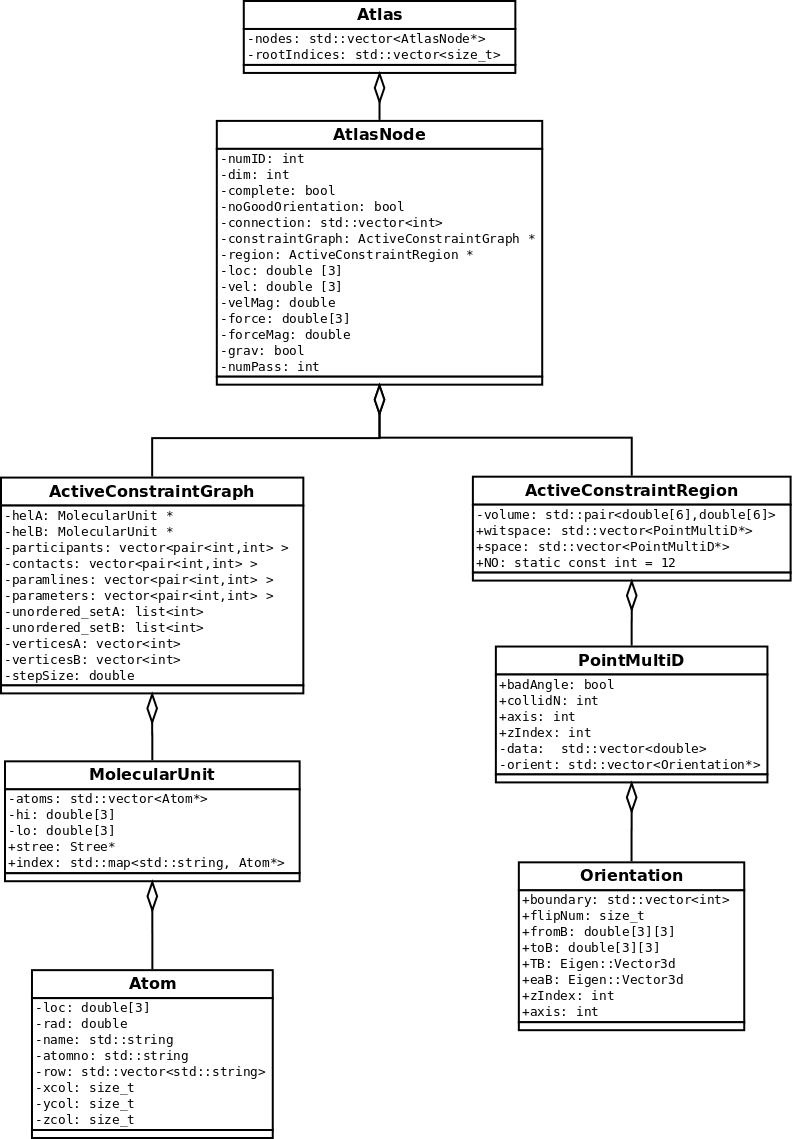
\includegraphics[scale=0.3] {fig/EASAL_UML.png}
\caption{EASAL UML Diagram}
\label{UML}
\end{figure}


\figref{UML} gives an overview of the structure of the major classes of EASAL.
Each of these classes are explained in the subsections below.

\subsubsection{AtlasBuilder} 

The AtlasBuilder class populates the ActiveConstraintRegion for each
activeConstraintGraph by sampling inside the boundaries of its ConvexChart. 
It creates and explores only regions that contain at least one Cartesian
realization. 

\begin{algorithm} [htbp]
 \SetKwInOut{Input}{input}\SetKwInOut{Output}{output}

 {\bf sampleAtlasNode}\\
 \Input{atlasNode: node}
 \Output{Complete sampling of the atlasNode and all its children}
 \BlankLine
 \LinesNumbered
	$H$ = node.activeConstraints\\
	$G_H$ = node.activeConstraintGraph\\
	\If{ $G_H$ is minimally rigid}
		{stop;	}
	$F$ = complete3Tree($G_H$)\\
	
	$C$ = computeConvexChart($G_H$, $F$)\\

	\For{ each cayleyPoint $p$ within convexChart $C$ }
	{
		$R$ = computeRealizations($p$)\\

		\For{ each realization $r$ in $R$}
		{
			\If{!aPosterioriConstraintViolated($r$)}
			{
				\If{ isBoundaryPoint($r$) \&\& hasNewActiveConstraint($r$, $G_H$) }
				{
					$e$ = newActiveConstraint($r$, $G_H$);\\
					$G'$ := $G_H \cup \{e\}$ ;\\
					\If{ $G'$ is not already present in the current atlas}
					{
						childNode = new atlasNode($G'$)\\
						sampleAtlasNode(childNode);\\
					} \Else{
						childNode = findNode($G'$);
					}
					node.setChildNode(childNode);
				} 
			}
		}
	}

	\caption{High level EASAL pseudocode}
\label{alg:sampleAtlasNode}
\end{algorithm}


\noindent \textbf{Major Attributes:} 
\begin{itemize}
		\item  \textbf{rootGraphs}: The set of all possible 4D or 5D
				ActiveConstraintGraphs of the root nodes
				generated before sampling.
		\item  \textbf{atlas}: An atlas object that is populated by the
				AtlasBuilder by sampling. This object is shared between front-end and
				back-end of the algorithm.
\end{itemize}

\noindent \textbf{Major Methods:}
\begin{itemize}
		\item  \textbf{startAtlasBuilding()}: For each of the generated root graph, 
				creates an atlasNode labeled with a contact graph $G_F$ where $F$ is the
				set of contacts. Then calls the recursive sampleTheNode method 
				for each of the root atlas nodes.
		\item  \textbf{sampleTheNode(atlasNode)}: The exploration of the atlas
				is done by the recursive \textbf{sampleAtlasNode} algorithm (see Algorithm 
				\ref{alg:sampleAtlasNode})
				using one of the generated atlas root nodes as input. This
				algorithm is implemented by the sampleTheNode method. Using
				depth first search this algorithm samples the atlas node and
				all its descendants. 
				
				\textbf{Base case of recursion:} If active constraint graph $G_H$ of the 
				node is minimally rigid i.e., the active constraint region is 
				0-dimensional, we have no more sampling to do, return.
				
				\textbf{The recursion step:} If $G_H$ is not minimally rigid, we use the
				\textbf{complete3Tree} algorithm to find find a set of parameters $F$ so 
				as to form a maximal 3-tree to leverage the convex parametrization theory~
				\cite{SiGa:2010}. This also ensures that $H \cup F$ is minimally rigid and 
				easily realizable. 
				
				The method computeConvexChart shown in the pseudocode finds the convex 
				chart for the parameters $F$ is done by the ConvexChart class explained 
				later. Method ComputeRealizations computes the realization for a 
				Cayley point and is done by the findRealizations method in the software. 
				The aPosterioriConstraintViolated method which checks for angle and steric 
				violations is implemented in the ConstraintCheck class explained later.
				Next we make a call to the findBoundary to detect boundaries and
				newly active constraints.
				

		\item  \textbf{determineStepSizeDynamically()}: Finds out the step size $s$
				given $T$, the total number of samples. Each 5D atlas node has its
				own $s$ computed by using the volume of the Cayley parameter space of the
				node over total number of samples per node. The volume of the
				Cayley parameter space of the node is approximately computed by
				exhaustive sampling within the exact chart without considering
				any constraints. The number of samples per node roughly can be
				computed by $T$ over total number of root(starter) atlas
				nodes, $m$. The number of samples in child nodes are negligible
				since the volume of regions in low dimensional nodes are
				negligible compared to the regions of high dimensional nodes.
		
		\item  \textbf{findBoundary()}: Boundary detection ensures that sampling 
				stays in the feasible region and minimizes discarded samples. 
				The findBoundary method which detects boundary points, checks 
				for newly formed active constraints and makes function calls
				which in turn call sampleTheNode for a child region.
		
\end{itemize}

\subsubsection{Atlas} 
The `Atlas' class stores the directed acyclic graph that represents the relationship between active constraint regions.

\noindent \textbf{Major Attributes:}
\begin{itemize}
		\item \textbf{nodes}: A vector of all AtlasNodes. 
		\item \textbf{rootIndices}: The indices of all the root nodes in the atlas.
\end{itemize}

\noindent \textbf{Major Methods:}
\begin{itemize}
		\item \textbf{search(node)}: Uses depth first search on the atlas to check
				whether the node exists in the atlas or not. It is used to avoid
				repeated sampling of the same region. The time complexity of
				the search is $O((\text{depth of the tree})) = O(6(k-1)) $ which in our 
				case is $O(1)$ since we fix $k$ to be 2.
\end{itemize}


\subsubsection{AtlasNode} 
AtlasNodes make up the Atlas. Each AtlasNode represents an active constraint region
reperesented by an ActiveConstraintGraph.

\noindent \textbf{Major Attributes:}
\begin{itemize}
		\item \textbf{acg}: The active constraint graph corresponding to the node.
		\item \textbf{region}: The set of Cayley points in the active region.
		\item \textbf{connection}: The id of the nodes in the atlas that
				represent the boundary of this node's region.
\end{itemize}

\subsubsection{ActiveConstraintGraph} 
The ActiveConstraintGraph class is used to store the set of active constraints.

\noindent \textbf{Major Attributes:} 
\begin{itemize}
		\item  \textbf{activeConstraints}: The set of point index pairs that represent 
				contacts.
		\item  \textbf{verticesA}: Participating points from first point set.
		\item  \textbf{verticesB}: Participating points from second point set.
		\item  \textbf{parameters}: A vector of point index pairs that represent parameters.
\end{itemize}

\noindent \textbf{Major Methods:}
\begin{itemize}
		\item  \textbf{completeTo3by3Graph()}: Adds points to make sure there
				are at least 3 points from each point set so that the graph is
				realizable. While choosing additional points, it has 2 options,
				choosing the points closest to each other or the points that lead
				to a user specified angle.
\end{itemize}


\subsubsection{ActiveConstraintRegion} 
The ActiveConstraintRegion class contains the set of feasible Cayley points generated
by sampling.

\noindent \textbf{Major Attributes:} 
\begin{itemize}
		\item  \textbf{space}: The set of feasible Cayley points.
		\item  \textbf{witspace}: The set of feasible witness Cayley points
				obtained from an ancestor node.
\end{itemize}

\noindent \textbf{Major Methods:}
\begin{itemize}
		\item  \textbf{convertSpace(activeConstraintRegion)}: Re-parametrizes
				a region using an input region’s parameters. This method
				converts each Cayley point in the input activeConstraintRegion
				to the Cayley point parametrized by the input region's
				parametrization.
\end{itemize}


\subsubsection{CayleyPoint} 
The CayleyPoint class represents a multi-dimensional point in the Cayley parameter space
and stores the corresponding Cartesian space orientations of the point set.

\noindent \textbf{Major Attributes:}
\begin{itemize}
		\item  \textbf{data}: Values of the Cayley parameters (non-edge
				lengths). \item  \textbf{orients}: The set of Cartesian space
				Orientations of the point set that were computed by
				realizing the active constraint graph with the given length of
				the edges and non-edges.
\end{itemize}

\subsubsection{Orientation} 
The Orientation class is the Euclidean transformation of point set. The
Orientation class stores only the information necessary to compute the
transformation matrix that will yield a Cartesian realization for the entire
point set.

\noindent \textbf{Major Attributes:} 
\begin{itemize}
		\item  \textbf{FromB}: Cartesian coordinates of three points from the
				first point set before the transformation.
		\item  \textbf{ToB}: Cartesian coordinates of three points from the
				second point set after the transformation.
		\item  \textbf{connections}: The set of node indices that this
				orientation belongs to. An orientation be on the
				boundary of multiple regions.
\end{itemize}


\subsubsection{CayleyParameterization} 
The CayleyParameterization class chooses non-edges in an ActiveConstraintGraph
that convert the graph into complete 3-tree. Those non-edges are called the
parameters. The complexity of the sampling algorithm varies based on the
choice of non-edges and the order in which they are fixed.

\noindent \textbf{Major Attributes:} 
\begin{itemize}
		\item  \textbf{partial3tree}: A boolean variable indicating whether
				an ActiveConstraintGraph is partial 3-tree or not.
		\item  \textbf{parameters}: The set of points pairs that represent
				non-edges. 
		\item  \textbf{tetrahedra}: The ordered tetrahedron set that helps in 
				defining the order of parameters that is required
				during the sampling procedure. This data is later passed to
				ConvexChart and CartesianRealizer to help in their computations. 
		\item  \textbf{updateList}: Adjacency map containing the dependency of
				parameters. It provides the set of parameters whose range will
				be updated when one of the parameters is fixed.
		\item  \textbf{boundaryComputationWay}: Inequalities that express the
				range of a parameter can be classified into either a linear or
				non-linear class. This variable is the characterization of the
				parameter that tells what inequality is needed to compute
				the parameter range i.e., triangular or tetrahedral inequality. 
		\item  \textbf{complete3trees}: The set of complete 3 trees.
\end{itemize}

\noindent \textbf{Major Methods:}
\begin{itemize}
		\item  \textbf{defineParameters()}: The parameters of an active
				constraint graph are selected as maximal 3-realizable (3-tree)
				extensions by leveraging the convex parametrization theory.
				\cite{SiGa:2010}. It creates a look-up table containing all possible 
				complete 3-trees. We find a graph in the look-up
				table so that active constraint graph is a proper subset of either the 
				graph or one of its isomorphisms.
		\item  \textbf{parameterMinDeviation()}: An alternate way to pick
				the parameters for 5D regions is by ensuring that the range
				of each parameter is similar. The aim here is to sample more
				uniformly in the Cartesian space. 
		\item  \textbf{built3tree()}: The 3-tree formed by starting with a
				4-vertex complete graph and repeatedly adding vertices in
				such a way that each added vertex is edge-connected to the face
				of a tetrahedron. Store the tetrahedrons in the order they are
				created in the attribute \textbf{tetrahedra}.
\end{itemize}


\subsubsection{ConvexChart} 

The ConvexChart class is used to determine the \chart\ that parameterize the
regions i.e., it computes the range of parameters of ActiveConstraintGraph. An
exact convex chart yields feasible Cayley points for the current active
constraint region. The resulting Cayley configuration space is convex, before
collisions or other (e.g.\ angle) constraints are introduced. The range of
parameters are computed by triangle and tetrahedral inequalities.

\noindent \textbf{Major Attributes:} 
\begin{itemize}
		\item  \textbf{param\_lengthUpper}: The upper bound of the parameters' range 
		\item  \textbf{param\_lengthLower}: The lower bound of the parameters' range 
		\item  \textbf{param\_length}: current value of parameters
\end{itemize}

\noindent \textbf{Major Methods:}
\begin{itemize}
		\item  \textbf{initializeChart()}: Initalizes the boundaries of
				convex chart. Tighter bounds are given in \cite{ugandhar}. 
		\item  \textbf{computeRange(v1, v2)}: Computes the range of the
				parameter $v1-v2$ in order to eliminate sampling infeasible grid
				points. Range computation is required in every iteration for
				dependent parameters. 
		\item  \textbf{setRangeByTriangleInequality(v1, v2)}: Computes the
				range of the non-edge $v1-v2$ through triangular inequalities.
		\item  \textbf{setRangeByTetrahedralInequality(v1, v2, tetrahedron)}:
				Computes the range of the non-edge $v1-v2$ through tetrahedral
				inequality.
		\item  \textbf{stepGrid}: Sets parameter point to the next grid point
				within the computed range.
		\item  \textbf{stepNeighbour()}: Sets the parameter point to the neighbor
				grid point in all dimensions consecutively.
		\item  \textbf{stepGridBinary()}: Sets the parameter point to 
				somewhere between current point and neighbor grid point
				according to binary search procedure in findBoundary.
\end{itemize}


\subsubsection{CartesianRealizer} 
The CartesianRealizer class contains routines that
compute orientations that represent transformations of rigid helices
relative to each other. It computes Cartesian realization of an active 
constraint graph with the
parameter lengths taken from cayleyPoint and active constraint lengths for a
specific flip. 
\noindent \textbf{Major Attributes:} 
\begin{itemize}
		\item \textbf{positions}: Cartesian coordinates of vertices in
				ActiveConstraintGraph.
		\item \textbf{edge\_length}: Contains all fixed distances plus current
				distance values of non-edges of ActiveConstraintGraph.
\end{itemize}

\noindent \textbf{Major Methods:}
\begin{itemize}
		\item  \textbf{computeRealization(activeConstraintGraph, convexChart,
				flipno)}: Computes the Orientation by leveraging partial 3-tree
				techniques. activeConstraintGraph which is a complete 3-tree is
				built up from a base tethedra by adding, at each step, a new
				vertex edge-connected to the face of a tetrahedron.
		\item  \textbf{setBaseTetra(tetrahedron)}: Finds Cartesian
				coordinates of the vertices of tetrahedron by known edge
				lengths.
		\item  \textbf{locateVertex(vertex, face)}: Finds Cartesian
				coordinates of the vertex that is connected to the face of a
				tetrahedron.
\end{itemize}


\subsubsection{ConstraintCheck} 

The ConstraintCheck class is designed to check whether any non-active
constraints become active. Users have the option
to define a set of constraints of interest. In which case, the new constraint
activation check is done only for these. For an input Orientation,
ConstraintCheck first computes the Cartesian realization for the entire \helix\
then passes it to other subroutines to perform user specified constraint check such as
steric constraints or angle constraints.
